%%==================================================
%% chapter01.tex for BIT Master Thesis
%% modified by yang yating
%% version: 0.1
%% last update: Dec 25th, 2016
%%==================================================
\chapter{绪论}
\enchapter{Introduction}
\label{chap:intro}
\section{研究背景及意义}
\ensection{Research Background and Motivation}

医疗器械研发是健康中国建设的重要内容。中共中央、国务院印发的《“健康中国2030”规划纲要》提出发展高性能医疗器械，提升新型制剂和高端医疗器械领域的创新能力\supercite{CPCStateCouncil2016HealthyChina}。国务院印发的《国民健康“十五五”规划》进一步提出加强医工协同，加大对高端医疗器械关键技术、元器件和整机研发的支持力度\supercite{StateCouncil2026NationalHealth}。

肝癌是我国恶性肿瘤防治的重点之一。国际癌症研究机构发布的 GLOBOCAN 2024 数据显示，2024 年全球肝癌新发病例估计约为 84.3 万例，死亡病例约为 73.2 万例，肝癌居全球癌症死因第三位\supercite{Sung2026GlobalCancer}。国家癌症中心估计，同期我国肝癌新发病例约为 35.4 万例，死亡病例约为 30.4 万例，肝癌居我国癌症死因第二位\supercite{Zheng2026CancerChina}。全球及我国的估计病例数见图~\ref{fig:liver-cancer-burden-2024}。经动脉化疗栓塞（transarterial chemoembolization，TACE）是肝细胞癌（hepatocellular carcinoma，HCC）局部介入治疗的常用手段，通过肿瘤供血动脉递送化疗药物并实施血管栓塞。随机对照研究在符合入组条件的不可切除 HCC 患者中观察到 TACE 的生存获益，我国《原发性肝癌诊疗指南（2026年版）》也将 TACE 纳入相应分期患者的治疗方案\supercite{Llovet2002Chemoembolisation,NHC2026LiverCancer}。欧洲肝脏研究学会指南及巴塞罗那肝癌分期策略均将 TACE 列为符合条件的患者的局部治疗选项，并强调结合肿瘤负荷、肝功能和选择性栓塞的可行性评估适用患者\supercite{EASL2025HCC,Reig2026BCLC}。

\begin{figure}[H]
  \centering
  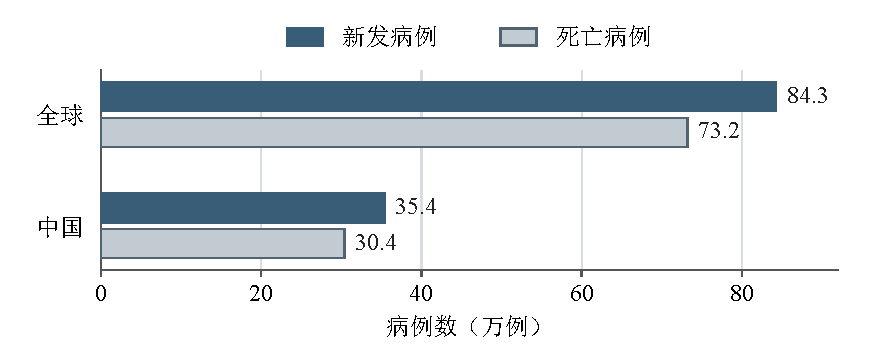
\includegraphics[width=0.85\textwidth]{figures/liver-cancer-burden-2024.pdf}
  \caption{2024 年全球及中国肝癌新发与死亡病例估计数\supercite{Sung2026GlobalCancer, Zheng2026CancerChina}}
  \label{fig:liver-cancer-burden-2024}
\end{figure}

传统碘油 TACE 通常将化疗药物水溶液与碘油混合成乳剂，再经导管输送至肿瘤供血动脉。由于油水两相不相溶，乳剂放置时可能发生液滴聚并或分层。实验研究表明，水相组成和油水比例会影响乳剂类型、物理稳定性及药物释放行为\supercite{Choi2014LipiodolEmulsions,Ahnfelt2019LipiodolEmulsions}。因此，如何在制备过程中改善药物的分散均匀性，并维持制剂在静置期间的物理稳定性，是碘油介入制剂开发中的工程问题。

超临界二氧化碳（supercritical carbon dioxide，scCO$_2$）的溶剂能力可通过调节温度和压力改变，降压后易于与产物分离，因而具有替代部分有机溶剂的潜力。已有研究涉及 scCO$_2$ 中增稠剂的溶解特性与增稠机理\supercite{Wang2024CO2Thickeners}、scCO$_2$ 及二氧化碳基混合工质在动力循环中的应用\supercite{Deng2025CO2PowerCycles}，以及利用 scCO$_2$ 从酸樱桃果核中提取脂质\supercite{Kniepkamp2024CherryStoneExtraction}。在 TACE 碘油制剂的制备中，可利用 scCO$_2$ 辅助混合，以改善药物在碘油中的分散状态和制剂的物理稳定性。

温度和压力是 scCO$_2$ 工艺的关键操作参数。在临界点附近，密度等热物性对温度和压力的变化较为敏感，进而影响流动和传热\supercite{Qing2025CarbonDioxideDensity,Zhang2024CO2HeatTransfer}。在植物种子油萃取研究中，Guta 等以种子油得率为优化目标，采用响应面法考察萃取温度、压力和时间的影响，并据此筛选工艺条件\supercite{Guta2025KorarimaExtraction}。对于碘油制剂的制备，需要根据目标药物在 scCO$_2$ 中的溶解特性筛选温压组合，并在混合过程中稳定维持所选条件，为重复制备和后续工艺放大提供基础。

基于上述需求，本文从制备设备和参数优化方法两方面开展研究。在设备方面，研制面向肝癌介入制剂制备的医疗器械，即智能超稳定均相混合系统，通过多路协同控制实现混合过程的自动化运行和温压精确调节。在参数优化方面，提出基于回归排序协同强化学习的端到端温压智能优化框架（SHIFT-TPO），以特定药物在 scCO$_2$ 中的溶解度最大化为目标，在设备允许的工况范围内筛选候选温压组合。两方面的研究为碘油制剂的工艺开发提供可重复的实验条件和参数选择依据。


\section{国内外研究现状}
\ensection{Research Progress Overview in Home and Abroad}

\subsection{超临界二氧化碳应用研究现状}
\ensubsection{Research Progress in Superstable Homogeneous Mixing Systems}
\label{subsec:shift-research-progress}

超临界二氧化碳在不同工艺中可承担萃取溶剂、抗溶剂、物理发泡剂或循环工质等作用。其在超稳定均相混合系统中的用途是辅助药物制备与分散，以获得均匀且具有一定物理稳定性的碘油制剂。与该系统直接相关的研究涉及两个方面：一是高压条件下的物料供给、温压调节与混合，二是卸压后制剂的分散状态及稳定性评价。

国外研究已将超临界二氧化碳应用于天然产物萃取、药物制备和纺织染整等领域。例如，Kniepkamp 等利用该介质从高含水酸樱桃果核中提取脂质，分析了原料含水量和预处理方式对萃取率的影响\supercite{Kniepkamp2024CherryStoneExtraction}。Mottola 等利用超临界抗溶剂沉淀法制备地塞米松和泼尼松龙的 $\beta$-环糊精包合物，以改善难溶药物的溶出性能\supercite{Mottola2024CorticosteroidSAS}。Broadbent 等则考察了染色温度、时间和助剂对聚酯纤维与二醋酸纤维上染、匀染的影响\supercite{Broadbent2026SupercriticalDyeing}。

在药物颗粒制备方面，Ha 等采用部分因子试验设计研究替米沙坦的超临界抗溶剂沉淀过程，发现药物溶液浓度和温度对颗粒粒径有显著影响\supercite{Ha2024TelmisartanSAS}。Sofia 等将超临界辅助制备与干燥集成，报告了脂质体粉末的粒径和包封率，并进行了中试放大\supercite{Sofia2025SupercriticalParticleFormation}。

在与混合系统相关的装置研究中，Dinh 等研制了高压二氧化碳--醇混合物物性测量装置。该装置可调节进料组成，在最高 $80\,^{\circ}\mathrm{C}$、$15.9\,\mathrm{MPa}$ 的测量范围内利用变容法和科里奥利密度计交叉验证混合物密度。作者在二氧化碳--乙醇体系中发现，混合不足可能造成密度测量偏差，说明进料比例和混合均匀性均需验证\supercite{Dinh2024HighPressureMixing}。日本的多孔玻璃膜乳化装置借助注射器往复推动碘油与药液穿过玻璃膜，形成水滴分布较均匀的油包水乳剂\supercite{Ono2026GlassMembrane}。Tanaka 等将其用于表柔比星--碘油乳剂的制备并开展多中心临床研究。两类装置分别提供了高压流体混合与碘油制剂制备的实例，评价指标涉及混合物物性以及乳滴分布\supercite{Tanaka2026GlassMembraneTrial}。

超临界二氧化碳循环装置的实验也为温压响应测试提供了参考。Kim 等在循环试验台上施加瞬态扰动，验证了带扰动观测器的压缩机入口温度控制策略\supercite{Kim2024CO2InletControl}。Huang 等在自然循环回路中观察到压降振荡，并分析了加热热流密度和稳压容积的位置对振荡的影响\supercite{Huang2024CO2PressureOscillation}。这两项研究所关注的温度跟踪和压力波动，可作为制备装置动态性能评价的参考指标。

\begin{figure}[!htbp]
  \centering
  \begin{subfigure}[t]{0.32\textwidth}
    \centering
    \parbox[c][35mm][c]{\linewidth}{\centering
      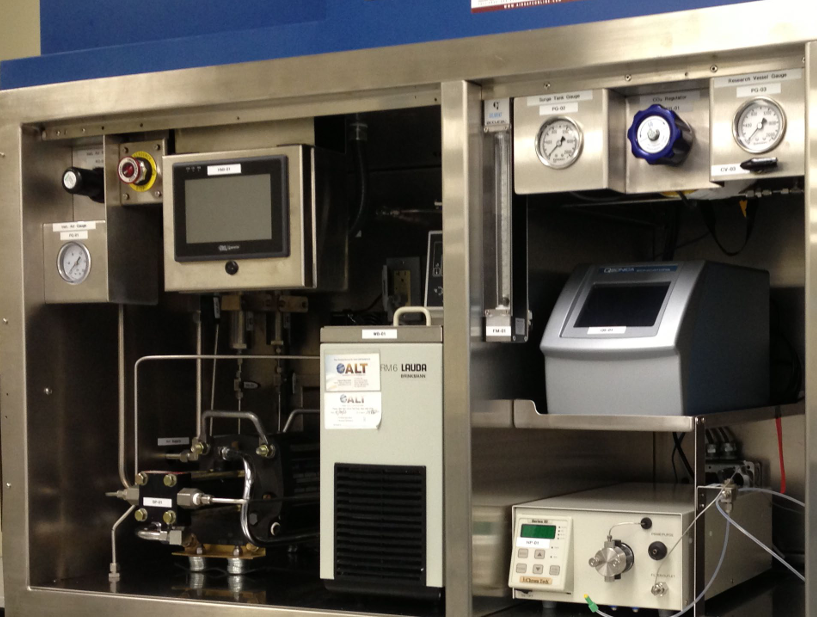
\includegraphics[width=\linewidth,height=35mm,keepaspectratio]{figures/equipment-crititech.png}}
    \caption{CritiTech Purcision 装置}
  \end{subfigure}\hfill
  \begin{subfigure}[t]{0.32\textwidth}
    \centering
    \parbox[c][35mm][c]{\linewidth}{\centering
      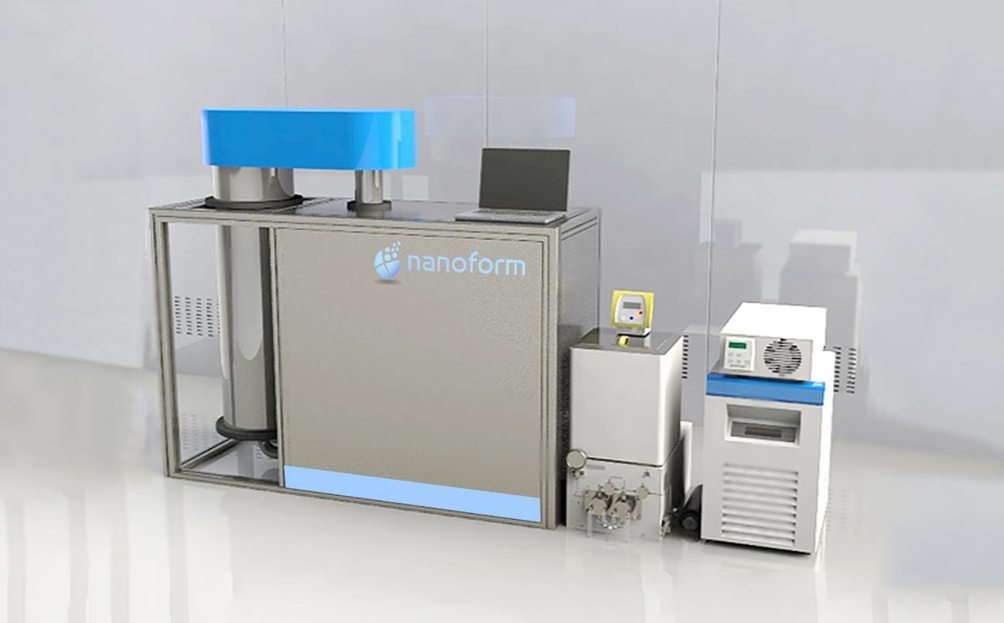
\includegraphics[width=\linewidth,height=35mm,keepaspectratio]{figures/equipment-nanoform.png}}
    \caption{Nanoform CESS 装置}
  \end{subfigure}\hfill
  \begin{subfigure}[t]{0.32\textwidth}
    \centering
    \parbox[c][35mm][c]{\linewidth}{\centering
      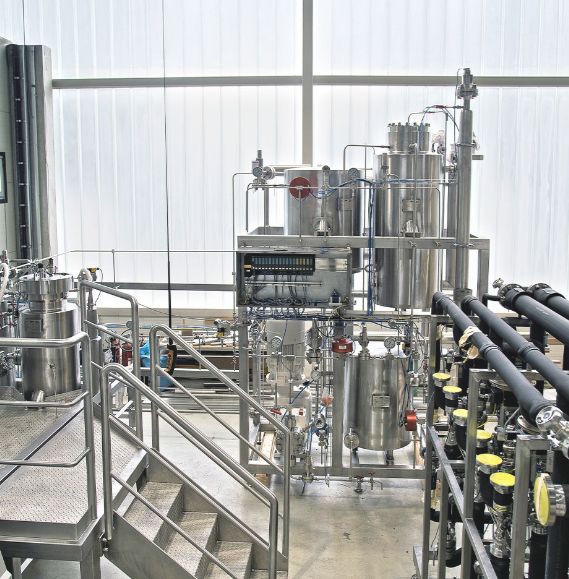
\includegraphics[width=\linewidth,height=35mm,keepaspectratio]{figures/equipment-natex.png}}
    \caption{Natex 制药萃取装置}
  \end{subfigure}
  \caption[国外超临界二氧化碳制药设备实例]{国外超临界二氧化碳制药设备实例\supercite{CritiTech2025PurcisionEquipment,NanoformCESSProcessLine,NatexPharmaceuticalEquipment}}
  \label{fig:foreign-supercritical-pharma-equipment}
\end{figure}

图~\ref{fig:foreign-supercritical-pharma-equipment} 展示了国外超临界二氧化碳制药设备的三个实例。美国 CritiTech 的 Purcision 装置采用超临界沉淀工艺制备药物颗粒\supercite{CritiTech2025PurcisionEquipment}。芬兰 Nanoform Finland Oyj 的 CESS 装置利用超临界溶液受控膨胀制备原料药纳米颗粒\supercite{NanoformCESSProcessLine}。奥地利 Natex Prozesstechnologie GesmbH 的工业萃取装置利用超临界二氧化碳从天然药用原料中提取活性成分\supercite{NatexPharmaceuticalEquipment}。

国内在食品加工、高分子发泡和介入制剂领域均开展了相关研究。董科等将超临界二氧化碳用于红花椒油树脂萃取，分析工艺参数与提取物风味组成之间的关系\supercite{Dong2025PepperOleoresin}。宫政等以超临界二氧化碳为发泡剂制备可降解形状记忆泡沫，考察聚乳酸含量对二氧化碳扩散、泡孔结构和形状记忆性能的影响\supercite{Gong2025PBATLAFoaming}。

图~\ref{fig:domestic-supercritical-pharma-equipment} 为国内设备实例。普萃超临界（广东）高新技术有限公司的实验型超临界纳米结晶设备用于药物颗粒制备\supercite{Zhu2025PucuiEquipment}。南通华达制药设备科技有限公司的超临界二氧化碳萃取设备可用于医药原料提取\supercite{HuadaSupercriticalExtractor}。

\begin{figure}[!htbp]
  \centering
  \begin{subfigure}[t]{0.46\textwidth}
    \centering
    \parbox[c][39mm][c]{\linewidth}{\centering
      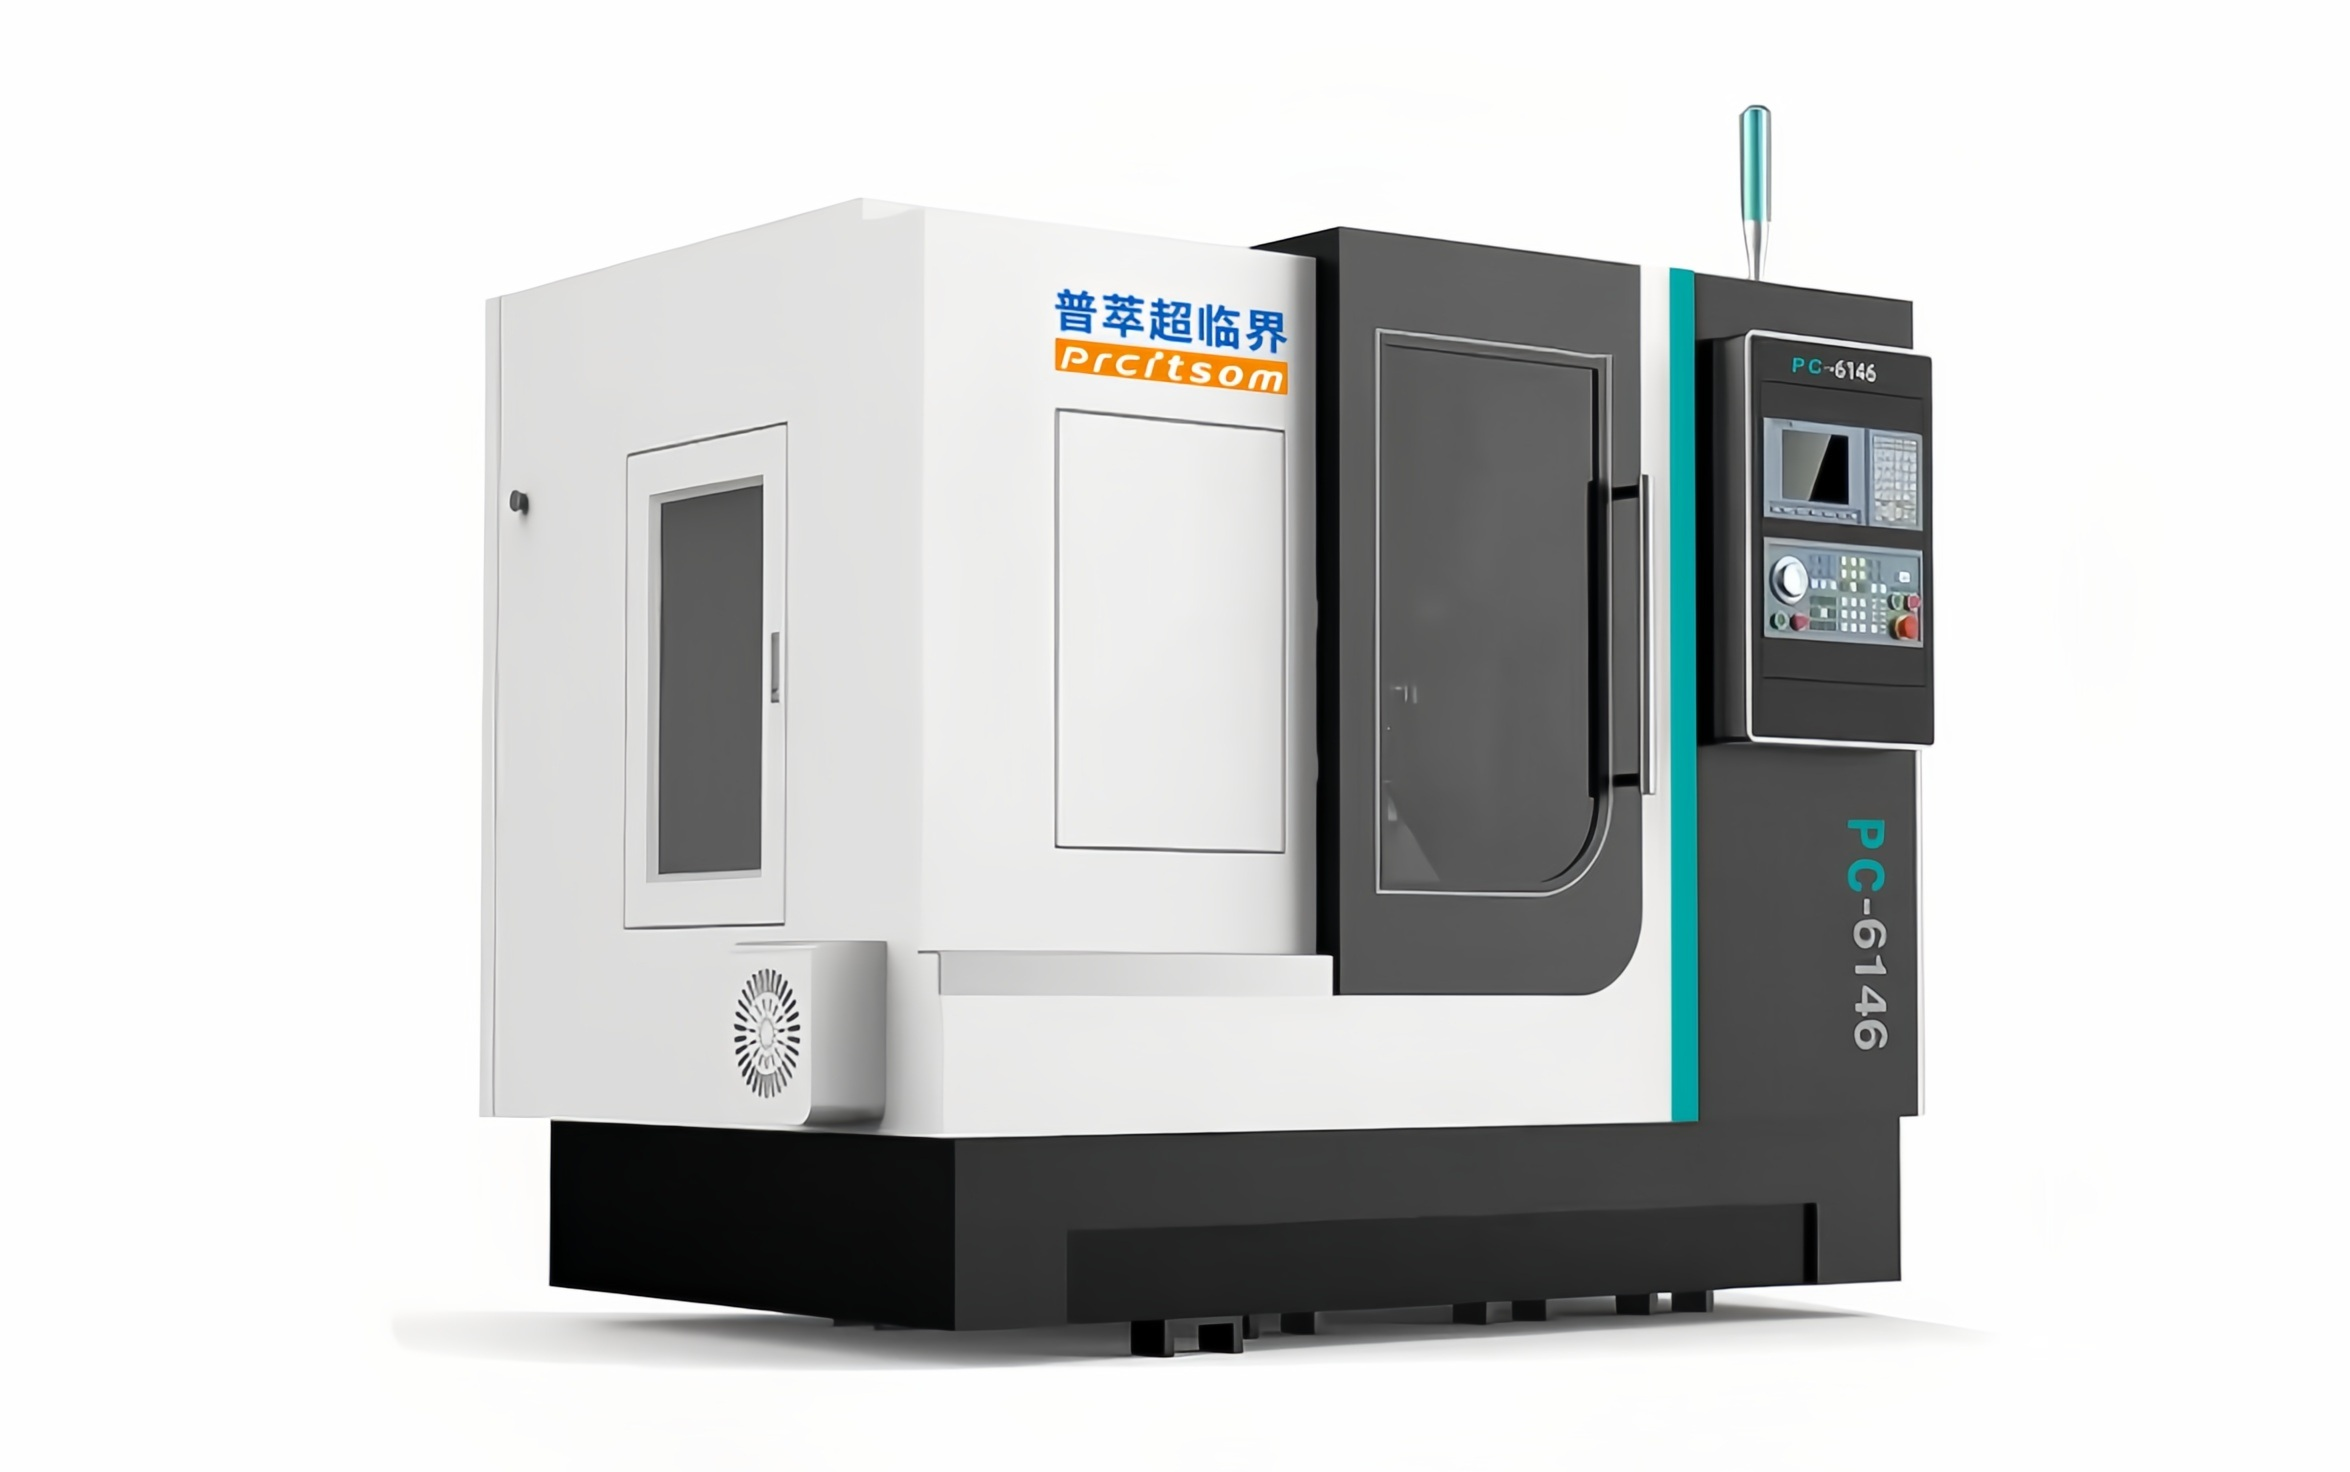
\includegraphics[width=\linewidth,height=39mm,keepaspectratio]{figures/equipment-pucui.png}}
    \caption{普萃超临界纳米结晶设备}
  \end{subfigure}\hfill
  \begin{subfigure}[t]{0.46\textwidth}
    \centering
    \parbox[c][39mm][c]{\linewidth}{\centering
      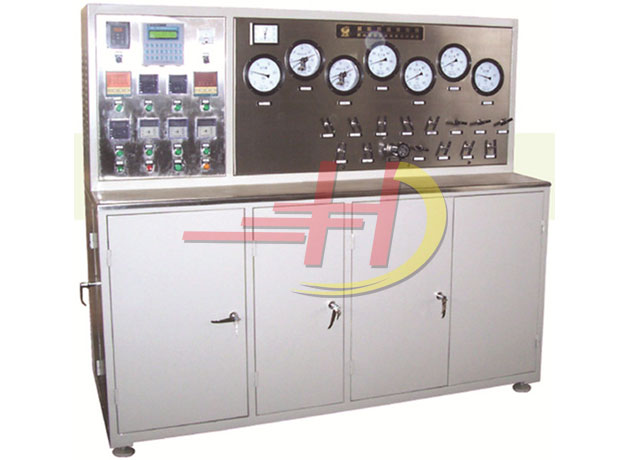
\includegraphics[width=\linewidth,height=39mm,keepaspectratio]{figures/equipment-nantong-huada.png}}
    \caption{南通华达超临界萃取设备}
  \end{subfigure}
  \caption[国内超临界二氧化碳制药设备实例]{国内超临界二氧化碳制药设备实例\supercite{Zhu2025PucuiEquipment,HuadaSupercriticalExtractor}}
  \label{fig:domestic-supercritical-pharma-equipment}
\end{figure}

在介入制剂领域，一类研究通过调整碘油乳剂的组成来延长药物释放或改善乳滴稳定性。Kim 等在动物实验中评价了温敏型碘油乳剂的局部递药效果\supercite{Kim2023IodizedOilEmulsion}。Wang 等与 Xia 等分别采用不同的颗粒稳定体系构建碘油 Pickering 乳剂，并开展了乳剂稳定性表征和动物实验\supercite{Wang2024LipiodolPickering,Xia2025LipiodolPickering}。

陈虎等于 2020 年报道了超稳定均相碘油配方技术（super-stable homogeneous intermixed formulation technology，SHIFT），实现吲哚菁绿（indocyanine green，ICG）在碘油中的稳定分散，并在兔肝肿瘤模型中验证了栓塞后荧光导航的可行性\supercite{Chen2020SHIFTS}。Zhang 等进一步在兔肝肿瘤模型中考察了纳米 ICG--碘油制剂对微小卫星灶的荧光显示\supercite{Zhang2022ShiftNanoICG}。Xiong 等报告了一例破裂性肝癌患者接受 SHIFT-ICG 栓塞后进行荧光引导切除的病例\supercite{Xiong2023ShiftRupturedHCC}。

\begin{figure}[!htbp]
  \centering
  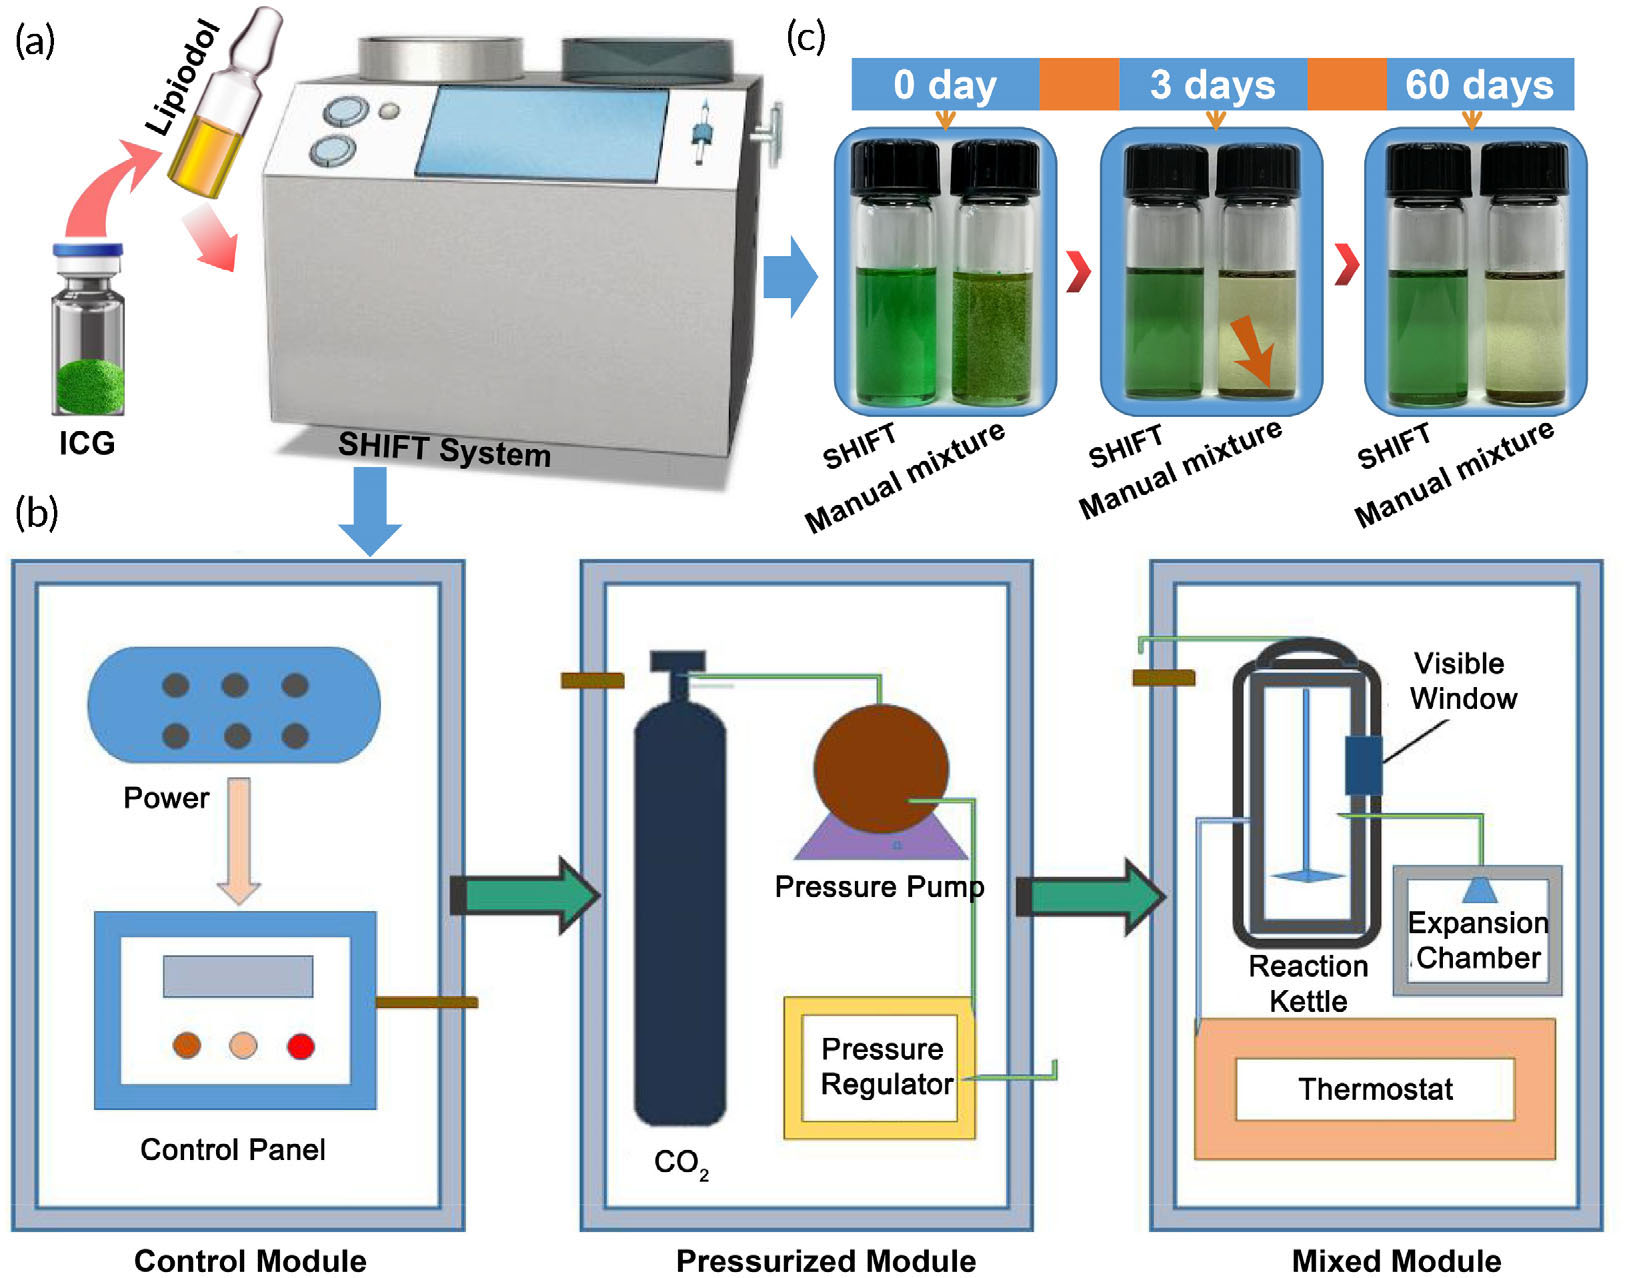
\includegraphics[width=0.83\textwidth]{figures/shift-prototype-stability.jpg}
  \caption{SHIFT 装置、功能模块及 ICG--碘油制剂静置对比\supercite{He2023SHIFTExploratory}}
  \label{fig:shift-prototype-stability}
\end{figure}

何攀等于 2023 年公开了面向碘油制剂的 SHIFT 装置。如图~\ref{fig:shift-prototype-stability} 所示，该装置由控制模块、加压模块和药物混合模块组成，可完成加料、制备、收集与清洗等操作。其制备的 ICG--碘油制剂在室温下静置 60~d 后仍未出现可见分层，并在一项纳入 45 例肝癌患者的回顾性研究中用于探索栓塞后荧光导航\supercite{He2023SHIFTExploratory}。在化疗制剂方面，何攀等先在超临界条件下制备纳米阿霉素，再将其超声分散于碘油中。所得制剂在 $25\,^{\circ}\mathrm{C}$ 下静置 21~d 后未见分层或沉淀\supercite{He2022SHIFTDOX}。此后，SHIFT 的应用拓展至替拉扎明与索拉非尼的双药碘油配方\supercite{Gao2025HomogeneousLipiodol}，以及已开展临床前和首次人体研究的放射性碘油配方\supercite{Chen2025Radiolipiodol}。

上述研究为碘油制剂制备提供了设备和工艺依据。现有 SHIFT 公开论文主要报告装置组成、代表性配方的制备条件及制剂表征，针对不同药物的适宜温压区间，以及升温升压、保温保压和卸压阶段的动态控制性能，仍需开展系统评价。对于包含纳米颗粒的碘油制剂，物理稳定性可通过颗粒分布、静置后分层或沉降等指标表征。基于这些研究，本文将设备的多路协同控制与候选温压组合筛选相结合，为后续制剂均匀性与批次重复性的验证提供可重复的制备条件。

\subsection{温压智能优化研究现状}
\ensubsection{Research Progress in Intelligent Temperature and Pressure Optimization}
\label{subsec:temperature-pressure-optimization}

在超稳定均相混合系统中，设备的温压控制负责跟踪设定值，工艺参数优化则负责确定适合目标药物的设定值。以药物在 scCO$_2$ 中的平衡溶解度作为筛选指标时，需要在设备允许的工况范围内联合选择温度和压力。温度对溶解度的影响随压力而变。升温会降低定压下的 scCO$_2$ 密度，同时提高固体溶质的升华蒸气压，两种效应共同决定溶解度的变化方向。Sodeifian 等测得帕博西尼在 scCO$_2$ 中的平衡溶解度，如图~\ref{fig:palbociclib-temperature-pressure} 所示，在 $18\,\mathrm{MPa}$ 时升温使溶解度降低，在 $21\,\mathrm{MPa}$ 时升温则使溶解度升高。由此可见，在单一压力下得到的温度效应难以直接推广至其他工况\supercite{Sodeifian2023Palbociclib}。

\begin{figure}[!htbp]
  \centering
  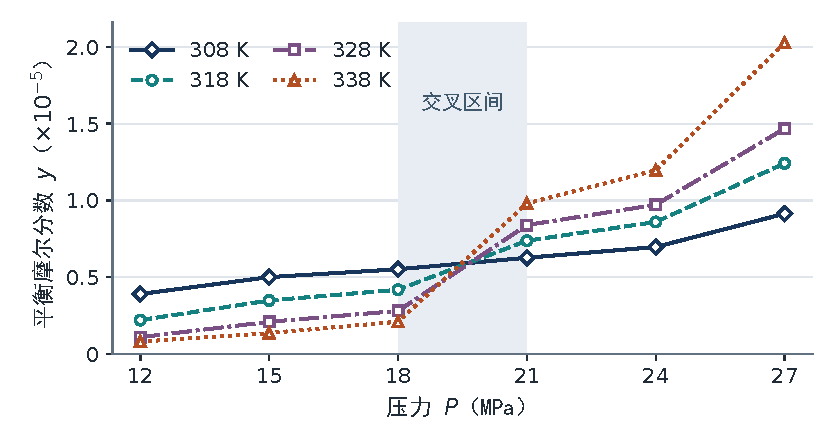
\includegraphics[width=0.86\textwidth]{figures/palbociclib-temperature-pressure.pdf}
  \caption{不同温度下帕博西尼在超临界二氧化碳中的平衡溶解度\supercite{Sodeifian2023Palbociclib}}
  \label{fig:palbociclib-temperature-pressure}
\end{figure}

（1）基于试验设计与热力学模型的参数筛选。响应面法通常先在选定的工况范围内安排试验，再用回归模型估计温度、压力等变量的主效应与交互作用。Guta 等采用 Box--Behnken 设计，以萃取温度、压力和时间为因子，获得了与实测得率相近的种子油得率预测值。国内刘国祎等在亚临界 CO$_2$ 萃取红花籽油的研究中，用同一批试验数据比较了响应面法与人工神经网络，并结合遗传算法搜索后者预测的高得率工况。这些研究说明，实验设计与模型搜索可以结合使用，但响应面及其最优点的适用性取决于物料和试验范围\supercite{Guta2025KorarimaExtraction,Liu2024SafflowerExtraction}。对于药物的平衡溶解度，Sodeifian 等采用 Peng--Robinson 状态方程描述帕博西尼与 CO$_2$ 的相平衡，利用实验数据校准模型参数。该方法可以根据相平衡关系解释操作条件对溶解度的影响，但对于缺少实测数据的药物，临界性质估算及相互作用参数的获取会限制模型应用\supercite{Sodeifian2023Palbociclib}。

在其他药物体系中，Ansari 等通过阿立哌唑的平衡溶解度测量识别了温度效应发生转变的压力区间\supercite{Ansari2023AripiprazoleSolubility}。Nateghi 等采用静态法测定尼洛替尼盐酸盐一水合物的溶解度，并在同一组实测数据上比较了经验关联式、状态方程和机器学习模型\supercite{Nateghi2023NilotinibSolubility}。

（2）基于数据驱动模型的溶解度预测。国内邵阳学院 Li 等以温度和压力为输入，比较了多项式回归、极端梯度提升和 LASSO 回归对氟尼酸溶解度及 scCO$_2$ 密度的预测表现。该研究以单种药物为对象，所用启发式算法优化的是模型超参数，其结果可作为工况筛选的预测依据\supercite{Li2024NiflumicAcid}。为使模型适用于多种溶质，Ji-En Li 等汇集了 116 种类药溶质的 2791 条数据，在温度、压力和 CO$_2$ 密度之外引入分子量和分子表面电荷密度分布，并比较了深度神经网络和随机森林的预测表现\supercite{Li2024MolecularSigmaProfiles}。

在分子特征构建方面，Roosta 等将原子贡献特征与机器学习结合，拟合多种固体药物的溶解度\supercite{Roosta2025DrugSolubility}。Sheikhshoaie 等利用药物热力学性质和工况变量比较了多种树模型\supercite{Sheikhshoaei2025DrugSolubility}。Makarov 等进一步整合了 31975 条溶解度记录，在梯度提升模型和分子图模型中加入熔点、汽化焓及溶剂化自由能等热力学信息，并按化合物分组评估模型对新分子的预测能力\supercite{Makarov2025ThermodynamicsInformedSolubility}。Khafagy 等使用七种药物的实验数据分析了分子描述符和工况变量对预测结果的影响，并指出部分实验记录缺少共溶剂信息，限制了模型对这类工艺差异的描述\supercite{Khafagy2026InterpretableSolubility}。

（3）基于搜索与策略学习的工况决策。图~\ref{fig:temperature-pressure-optimization-workflows} 对比了响应面优化、固定代理模型搜索和序贯实验优化的基本流程。采用固定代理模型时，可利用已有数据拟合溶解度，再在设备范围内通过网格搜索或遗传算法选择候选点。Trabucco 等提出的 Design-Bench 为仅使用历史数据的离线优化方法提供了统一测试任务\supercite{Trabucco2022DesignBench}。Tan 等在离线优化基准上发现，代理模型维持候选方案相对顺序的能力与寻优表现的关联强于均方误差，并据此采用排序学习筛选候选方案\supercite{Tan2025OfflineRanking}。对于溶解度模型，若个别工况的估计值偏高，搜索结果可能偏离实测溶解度较高的区域。因此，模型的总体回归精度和识别高溶解度工况的能力需要分别评价。

\begin{figure}[!htbp]
  \centering
  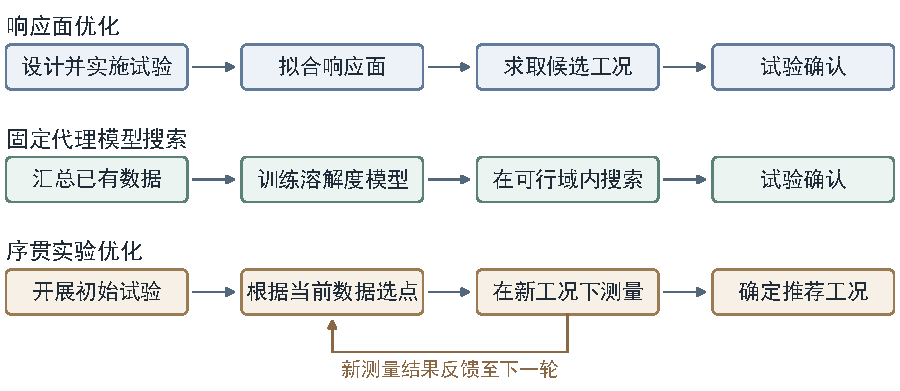
\includegraphics[width=0.97\textwidth]{figures/temperature-pressure-optimization-workflows.pdf}
  \caption{工艺参数优化的典型流程}
  \label{fig:temperature-pressure-optimization-workflows}
\end{figure}

采用序贯实验优化时，每轮将新测量结果反馈给模型或搜索算法，用于选择下一组工况。Florit 等将贝叶斯优化与动态流动实验结合，并在酯水解反应中验证了该流程\supercite{Florit2025DynamicFlowBayes}。Taylor 等利用相关反应的历史数据初始化多任务贝叶斯优化，并在连续流反应平台上验证了该方法\supercite{Taylor2023MultitaskOptimization}。Wang 等利用多臂赌博机算法依据实验反馈分配采样次数，在三类反应中使用不足预设反应空间 $15\%$ 的样本识别出适用于多种底物的反应条件\supercite{Wang2024BanditReaction}。对于需要达到平衡后取样的 scCO$_2$ 高压实验，逐轮更新的成本还取决于单次测量时间与可用实验次数。

强化学习也被用于具有反馈的工艺决策。McClement 等在仿真环境中训练策略，用于在线调整比例积分控制器参数\supercite{McClement2022MetaRLPI}。Petsagkourakis 等在含模型不确定性的过程控制算例中引入机会约束，以概率形式描述运行约束\supercite{Petsagkourakis2022ChanceConstrainedPolicy}。国内 Lou 等将近端策略优化用于药物洗脱支架的药物扩散调节，以治疗区域内的药物浓度与均匀性等指标评价策略，并比较了不同支架嵌入构型下的表现\supercite{Lou2026StentDiffusionRL}。对于 SHIFT 的平衡温压筛选，在组分和工况给定后，可用该条件下的平衡溶解度评价一次决策。基于历史数据构建奖励模型，可以减少策略训练对反复开展高压实验的依赖。

已有研究为超临界工艺提供了相平衡计算、溶解度预测与实验选点方法。针对 SHIFT 中的药物工况筛选，仍需考察模型在未见药物和设备可行域收窄时，能否识别相对优良的温压组合。药物在 scCO$_2$ 中的平衡溶解度可作为初筛目标，卸压后在碘油中的分散均匀性和静置稳定性则需要通过制剂实验评价。基于上述研究，本文将给定药物和可行工况范围下的平衡温压筛选建模为单步决策，利用溶解度回归与工况排序共同构建奖励模型，并训练策略生成候选温压组合，为后续混合实验提供设定值。

\section{存在的问题}
\ensection{Existing Problems}

现有 SHIFT 装置已用于多种碘油制剂的制备，公开研究主要报告装置组成、代表性配方的制备条件及所得制剂的物理稳定性。在实际制备过程中，升温升压、保温保压和卸压各阶段对温压调节与气路切换的要求不同。尤其在升温升压阶段，加热和进气均可能改变混合腔内的压力，需要协调加热、供气与阀门动作。现有公开报道对各阶段的温压响应和稳定性描述较少，难以据此判断设备能否在不同设定条件下达到并维持目标温度和压力。如何使各工序按预定条件运行，并减小相同设定值下的批次间温压差异，是提高制备过程重复性需要解决的问题。

不同药物在 scCO$_2$ 中的溶解特性存在差异，且温度对溶解度的影响可能随压力变化，已有配方的温压参数难以直接用于其他药物。逐组测定平衡溶解度需要在各温压条件下等待体系达到平衡后再取样，因而筛选多个工况的实验周期较长。现有数据驱动模型能够依据药物与工况特征预测溶解度。将预测结果用于温压筛选时，个别工况的估计偏差就可能改变候选组合的排序。对于训练数据未覆盖的药物，尤其是在设备允许的温压范围较窄时，如何从可行工况中识别溶解度较高的温压组合，仍需进一步研究。

基于上述问题，本文开展智能超稳定均相混合系统设计、制备过程自动控制与温压参数优化研究，并结合系统集成与混药实验，考察设备对设定工况的执行情况以及所得制剂的分散状态与静置稳定性。

\section{主要研究内容}
\ensection{Major Contents and Chapter Arrangement}

面向肝癌介入用碘油制剂的制备需求，本文研制智能超稳定均相混合系统，并研究不同药物的工艺温压筛选方法。系统按照给定的温度和压力控制混合过程，优化模型依据药物特征和允许的工况范围推荐候选温压组合。研究内容包括：

（1）设计智能超稳定均相混合系统的总体方案。结合加料、升温升压、保温保压和卸压等工序，分析机械结构、温压调节和操作环境的设计需求，确定混合装置与气路的布置、上下位机的功能分工以及温压优化模型的输入与输出。在此基础上，完成上位机、主控芯片、气路阀门、温压检测与调节模块以及超净台相关部件的选型。

（2）设计并实现混合设备的控制系统。围绕温压信号采集和执行机构驱动，设计供电、RS-485 通信、开关驱动及模数和数模转换电路。下位机实现温度与压力调节、状态监测、二氧化碳检测、卸压及 PID 参数自整定等功能。上位机通过串口与下位机交换控制指令及运行数据，实现工艺参数设置、运行状态显示和设备操作。

（3）提出基于回归排序协同强化学习的端到端温压优化框架 SHIFT-TPO。以目标药物在 scCO$_2$ 中的平衡溶解度最大化为目标，将温压组合选择建模为单步马尔可夫决策过程。构建回归排序协同网络（RRCN）作为奖励模型，融合分子结构、分子物性和工况特征，同时学习溶解度数值与不同工况下溶解度的相对排序。采用近端策略优化（PPO）算法训练温压推荐策略，并在奖励函数中以软约束纳入设备允许的温压范围。通过对比实验、消融实验和物理可解释性分析，考察模型的温压寻优性能及其在未见药物和受限工况下的表现。

（4）开展系统集成与应用实验。完成混合装置、温压调节部件和控制系统的集成调试，通过混药实验考察设备运行、制剂分散状态和静置稳定性。结合具体药物与设备工况，分析模型推荐的温压组合在混药实验中的适用性。
